% The Hilbert curve of orders 1, 2 and 3 over a square frame: the order in which numbers are laid out.
\documentclass[tikz,border=2mm]{standalone}
\usepackage{fontspec}\setmainfont{LibertinusSans}[Extension=.otf,UprightFont=*-Regular,BoldFont=*-Bold,ItalicFont=*-Italic]
\usepackage{pgfplots}\pgfplotsset{compat=1.18}
\usepackage{pgfplotstable}
\definecolor{ink}{HTML}{A3121C}\definecolor{inkmid}{HTML}{D9584F}\definecolor{inklight}{HTML}{F2B8B3}\definecolor{inkpale}{HTML}{FBE3E1}
\definecolor{slate}{HTML}{8C9AA6}\definecolor{grid}{HTML}{DADDE0}
\providecommand{\T}[2]{\ifdefined\paperfr #2\else #1\fi}
\usetikzlibrary{lindenmayersystems}
\begin{document}
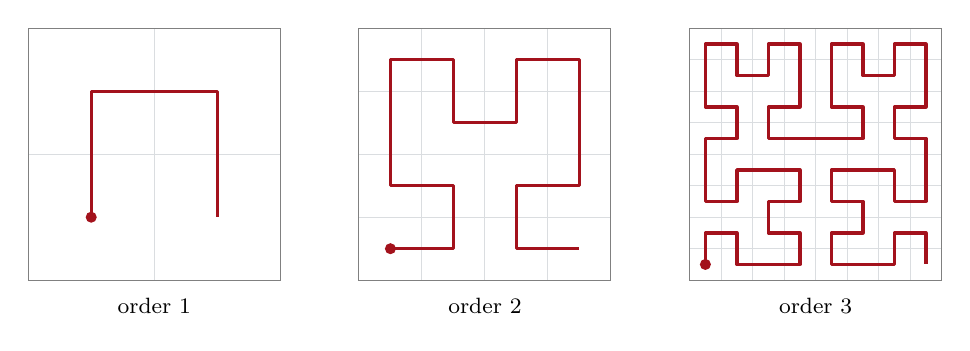
\begin{tikzpicture}[font=\footnotesize]
\foreach \k/\s [count=\i from 0] in {1/1.6,2/0.8,3/0.4} {
  \begin{scope}[xshift=\i*4.2cm]
    \draw[grid, step=\s] (0,0) grid (3.2,3.2);
    \draw[gray] (0,0) rectangle (3.2,3.2);
    \begin{scope}[shift={(\s/2,\s/2)}]
      \draw[ink, very thick, line join=round] [l-system={rule set={L -> +RF-LFL-FR+, R -> -LF+RFR+FL-}, axiom=L, order=\k, step=\s cm, angle=90}] lindenmayer system;
    \end{scope}
    \fill[ink] (\s/2,\s/2) circle (2pt);
    \node[below] at (1.6,-0.1) {\T{order}{ordre} \k};
  \end{scope}}
\end{tikzpicture}
\end{document}
